\documentclass[12pt]{article}
\usepackage{graphicx,import}
\usepackage[svgnames]{xcolor} 
\usepackage{fancyhdr}
\usepackage{subfig}
\usepackage{hyperref}
\usepackage{enumitem}
\usepackage{cite}
\usepackage{fancyvrb}
\usepackage[many]{tcolorbox}
\usepackage{listings }
\usepackage[a4paper, total={6in, 8in} , bottom = 25mm , top = 25mm, headheight = 1.25cm , includehead,includefoot,heightrounded ]{geometry}
\usepackage{afterpage}
\usepackage{amssymb}
\usepackage{pdflscape}
\usepackage{gensymb}
\usepackage{textcomp}
\usepackage{tikz,pgfplots}
\usepackage{xecolor}
\usepackage{rotating}
\usepackage{pdfpages}
\usepackage[Kashida]{xepersian}
\usepackage[T1]{fontenc}
\usepackage{tikz}
\usepackage[utf8]{inputenc}
\usepackage{PTSerif} 
\usepackage{seqsplit}

\usepackage[edges]{forest}

\usepackage{listings}
\usepackage{xcolor}

\hypersetup{
	colorlinks   = true, %Colours links instead of ugly boxes
	urlcolor     = blue, %Colour for external hyperlinks
	linkcolor    = blue, %Colour of internal links
	citecolor   = red %Colour of citations
}
 
\definecolor{codegreen}{rgb}{0,0.6,0}
\definecolor{codegray}{rgb}{0.5,0.5,0.5}
\definecolor{codepurple}{rgb}{0.58,0,0.82}
\definecolor{backcolour}{rgb}{0.95,0.95,0.92}
 
\NewDocumentCommand{\codeword}{v}{
\texttt{\textcolor{blue}{#1}}
}
\lstset{language=java,keywordstyle={\bfseries \color{blue}}}

\lstdefinestyle{mystyle}{
    backgroundcolor=\color{backcolour},   
    commentstyle=\color{codegreen},
    keywordstyle=\color{magenta},
    numberstyle=\tiny\color{codegray},
    stringstyle=\color{codepurple},
    basicstyle=\ttfamily\normalsize,
    breakatwhitespace=false,         
    breaklines=true,                 
    captionpos=b,                    
    keepspaces=true,                 
    numbers=left,                    
    numbersep=5pt,                  
    showspaces=false,                
    showstringspaces=false,
    showtabs=false,                  
    tabsize=2
}

\lstset{style=mystyle}

\settextfont[Scale=1.2 ,BoldFont={Bahij Nazanin-Bold.ttf} , ItalicFont = {IRNazaninIranic.ttf}]{Bahij Nazanin-Regular.ttf}
\setlatintextfont[Scale = 1.0]{Garamond}
\DefaultMathsDigits 
\DeclareMathSizes{11}{19}{13}{9} 
%\DeclareMathSizes{12}{14.4}{8}{9}





\newenvironment{changemargin}[2]{%
\begin{list}{}{%
\setlength{\topsep}{0pt}%
\setlength{\leftmargin}{#1}%
\setlength{\rightmargin}{#2}%
\setlength{\listparindent}{\parindent}%
\setlength{\itemindent}{\parindent}%
\setlength{\parsep}{\parskip}%
}%
\item[]}{\end{list}}


\definecolor{foldercolor}{RGB}{124,166,198}

\tikzset{pics/folder/.style={code={%
    \node[inner sep=0pt, minimum size=#1](-foldericon){};
    \node[folder style, inner sep=0pt, minimum width=0.3*#1, minimum height=0.6*#1, above right, xshift=0.05*#1] at (-foldericon.west){};
    \node[folder style, inner sep=0pt, minimum size=#1] at (-foldericon.center){};}
    },
    pics/folder/.default={20pt},
    folder style/.style={draw=foldercolor!80!black,top color=foldercolor!40,bottom color=foldercolor}
}

\forestset{is file/.style={edge path'/.expanded={%
        ([xshift=\forestregister{folder indent}]!u.parent anchor) |- (.child anchor)},
        inner sep=1pt},
    this folder size/.style={edge path'/.expanded={%
        ([xshift=\forestregister{folder indent}]!u.parent anchor) |- (.child anchor) pic[solid]{folder=#1}}, inner xsep=0.6*#1},
    folder tree indent/.style={before computing xy={l=#1}},
    folder icons/.style={folder, this folder size=#1, folder tree indent=3*#1},
    folder icons/.default={12pt},
}

\begin{document}


%%% title pages
\begin{titlepage}
\begin{center}
        
\vspace*{0.7cm}


\includegraphics[width=0.4\textwidth]{sharif1.png}\\
\vspace{0.5cm}
\textbf{ \Huge{\emph ‌سیگنال‌ها و سیستم‌ها} }\\
\vspace{0.5cm}
\textbf{ \Large{ تمرین پنجم} }
\vspace{0.2cm}
       
 
      \large \textbf{دانشکده مهندسی کامپیوتر}\\\vspace{0.2cm}
    \large   دانشگاه صنعتی شریف\\\vspace{0.2cm}
       \large   ﻧﯿﻢ سال دوم 00-99 \\\vspace{0.2cm}
      \noindent\rule[1ex]{\linewidth}{1pt}
استاد:\\
    \textbf{{جناب آقای دکتر منظوری شلمانی}}


    \vspace{0.15cm}
نام و نام خانوادگی:\\

       
    \textbf{{امیرمهدی نامجو - 97107212}}
\end{center}
\end{titlepage}
%%% title pages


%%% header of pages
\newpage
\pagestyle{fancy}
\fancyhf{}
\fancyfoot{}
\cfoot{\thepage}
\chead{تمرین پنجم}
\rhead{
\includegraphics[width=0.1\textwidth]{sharif.png}}
\lhead{امیرمهدی نامجو}
%%% header of pages

\KashidaOff

\section{سری فوریه}
\subsection{سوال اول}

\subsubsection{بخش a}


$$
f(x)=\left\{\begin{array}{lr}
	\pi-x & 0 \leq x \leq \pi \\
	x-\pi & -\pi \leq x \leq 0
\end{array}\right.
$$

ابتدا عامل DC را بدست می‌آوریم:

$$a_0 = \frac{1}{2\pi} \int f(x) dx = \frac{1}{2\pi} \int_{-\pi}^{0} (x- \pi) dx + \int_{0}^{\pi} (\pi -x) dx$$
$$= \frac{1}{2\pi} (\frac{-3\pi^2}{2} - \frac{\pi^2}{2}) = \boxed{- \pi} $$

برای ضرایب کسینوسی داریم:

$$a_n = \frac{1}{\pi} \int (f(x) \cos (nx)) dx$$

$$= \frac{1}{\pi} (\int_{-\pi}^{0} (x - \pi) \cos (nx) dx + \int_{0}^{\pi} (\pi - x) \cos (nx) dx)$$

ابتدا لازم است اشاره کنیم که
$$\int x \cos (nx) = \frac{1}{n^2} \cos(nx) + \frac{1}{n} x \sin (nx)$$

با توجه به این موضوع، از عبارت بالا می‌توان به راحتی انتگرال گرفت:


$$= \frac{1}{\pi}( (\frac{\cos (n x)}{n^2}+\frac{x \sin (n x)}{n}-\frac{\pi  \sin (n x)}{n}) |_{-\pi}^{0} + (-\frac{\cos (n x)}{n^2}+\frac{\pi  \sin (n x)}{n}-\frac{x \sin (n x)}{n})|_{0}^{\infty})$$

بعد از ساده سازی و محاسبات داریم:

$$\boxed{a_n = -\frac{2 (\pi  n \sin (\pi  n)+\cos (\pi  n)-1)}{\pi  n^2} = \frac{-2((-1)^n -1)}{\pi n^2}}$$


برای محاسبات ضریب سینوسی داریم:

$$b_n = \frac{1}{\pi} \int (f(x) sin(nx)) dx$$

$$= \frac{1}{\pi} (\int_{-\pi}^{0} (x - \pi) \sin (nx) dx + \int_{0}^{\pi} (\pi - x) \sin (nx) dx)$$


ابتدا لازم است اشاره کنیم که
$$\int x \sin(nx) = \frac{\sin (n x)}{n^2}-\frac{x \cos (n x)}{n}  $$

با توجه به این موضوع، عبارت بالا مانند بخش قبل به راحتی قابل محاسبه است. جوابی که در نهایت به آن می رسیم به صورت زیر است:


$$\boxed{b_n = \frac{2-2 \cos (\pi  n)}{n} = \frac{2 - 2 (-1)^n}{n}}$$


و جواب نهایی به صورت:

$$f(x) = a_0 + \sum_{n=1}^{N} (a_n \cos (n x) + b_n \sin (n x))$$

خواهد بود. (تقسیم بر ۲ فرمول $a_0$ را به نوعی در خود انتگرال آن تاثیر داده‌ام)

کد آن در فایل 
\lr{\Verb+P1\_Q1\_a.py+}
قرار دارد. نمودار در صفحه بعد قرار گرفته است. شکل بالایی خود تابع و شکل های بعدی به ازای $N=2,5,20,50$ هستند.

\begin{center}
	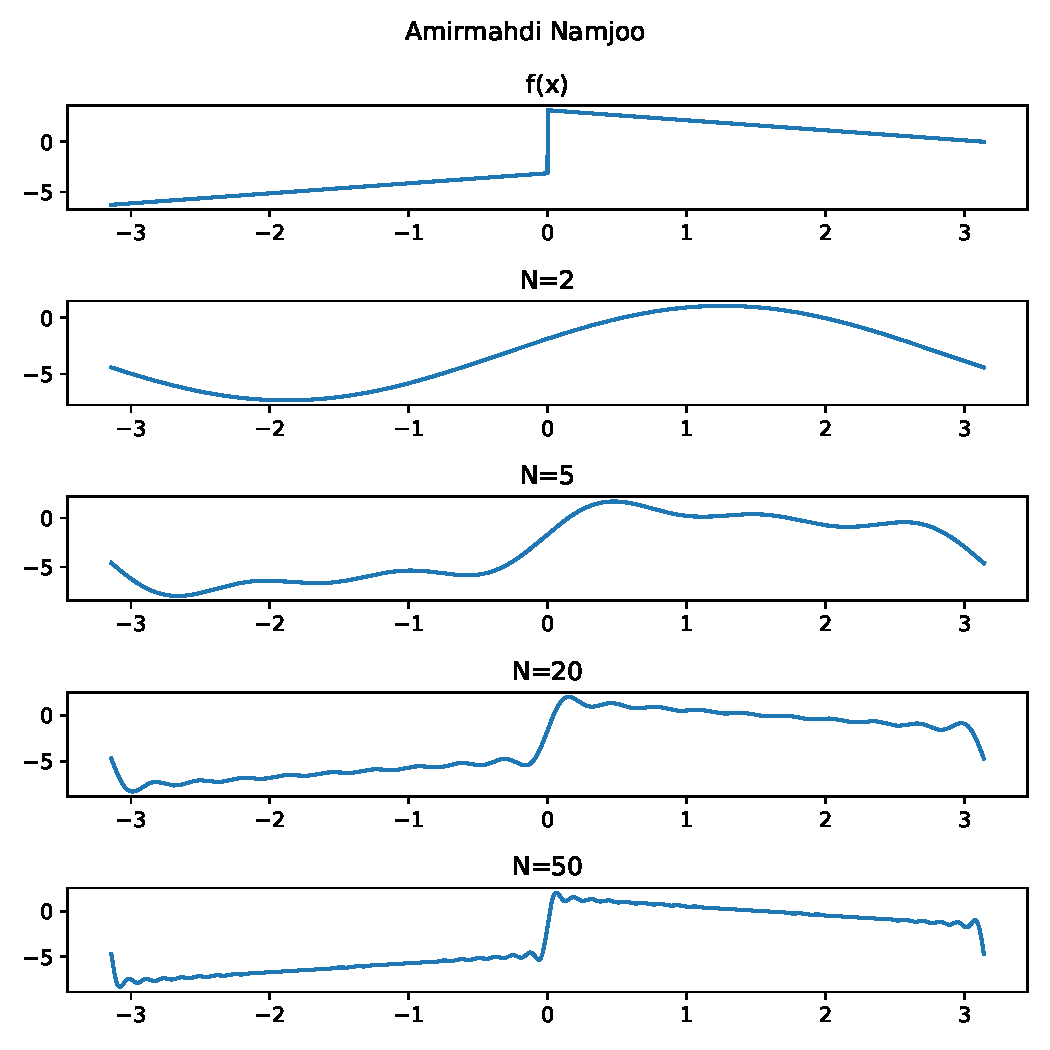
\includegraphics[width = 1.0 \textwidth]{images/1.pdf}
\end{center}


\newpage

\subsubsection{بخش b}

$$
f(x)=\left\{\begin{array}{lr}
	1 & 0 \leq x<\frac{\pi}{2} \\
	0 & \frac{\pi}{2} \leq x<\pi \\
	0 & -\pi \leq x<0
\end{array}\right.
$$

$$a_0 = \frac{1}{2\pi} \int f(x) dx = \frac{1}{2\pi} \int_{0}^{\pi/2} 1 dx = \boxed{ \frac{1}{4}}$$


$$a_n = \frac{1}{\pi} \int (f(x) \cos (nx)) dx$$

$$=\frac{1}{\pi}\int_{0}^{\pi/2} \cos (nx) dx = \frac{1}{\pi }\frac{\sin(nx)}{n}|_{0}^{\pi/2}  = \boxed{\frac{\sin \left(\frac{\pi  n}{2}\right)}{\pi  n}}$$

$$b_n = \frac{1}{\pi} \int (f(x) \sin (nx)) dx$$
$$= \frac{1}{\pi} \int_{0}^{\pi/2} \sin (nx) dx = - \frac{1}{\pi} \frac{\cos (n x)}{n} |_{0}^{\pi/2}  = \boxed{\frac{2 \sin ^2\left(\frac{\pi  n}{4}\right)}{\pi  n}}$$

که در بالا از اتحاد
$\cos(2 \theta) = 1 - 2\sin^2 (\theta)$
استفاده شده است.


و جواب نهایی به صورت:

$$f(x) = a_0 + \sum_{n=1}^{N} (a_n \cos (n x) + b_n \sin (n x))$$



کد آن در فایل 
\lr{\Verb+P1\_Q1\_b.py+}
قرار دارد. نمودار در صفحه بعد قرار گرفته است. شکل بالایی خود تابع و شکل های بعدی به ازای $N=2,5,20,50$ هستند.

\begin{center}
	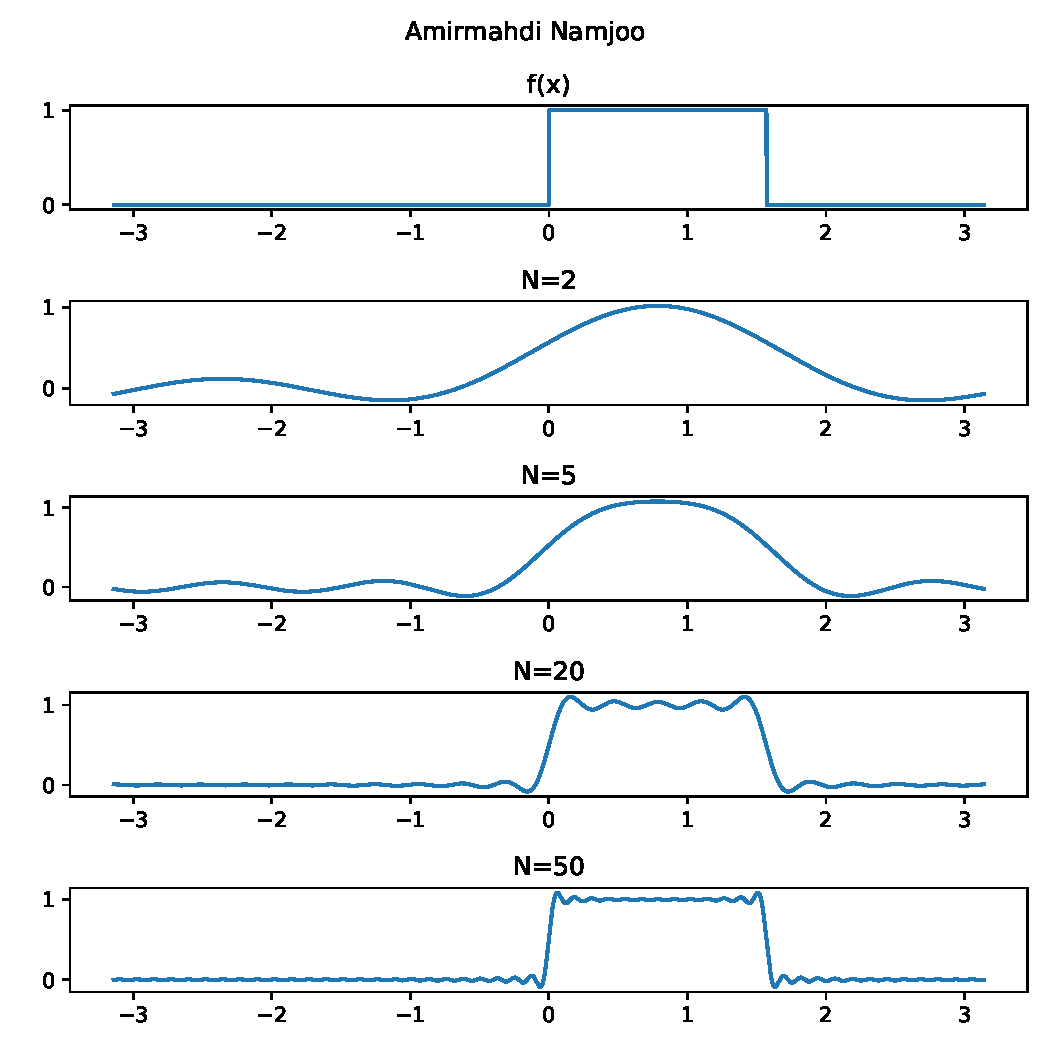
\includegraphics[width = 1.0 \textwidth]{images/2.pdf}
\end{center}

\newpage
\subsection{سوال دوم}
\subsubsection{بخش a}

$$\cos(4t) = \frac{1}{2} e^{-4 j t}+\frac{1}{2} e^{4 j t} $$

$$\sin(6t) = \frac{1}{2j} e^{6 j t}-\frac{1}{2j} e^{-6 j t} $$

در نتیجه ضرایب سری فوریه برای 
$\cos(4t)+\sin(6t)$
به صورت زیر است:

$$a_4 = \frac{1}{2} , a_{-4} = \frac{1}{2} , a_{6} = \frac{1}{2 j} , a_{-6} = \frac{-1}{2j}$$
و به ازای $k\neq \pm4,\pm6$ داریم $a_k = 0$

\subsubsection{بخش b}
\begin{center}
	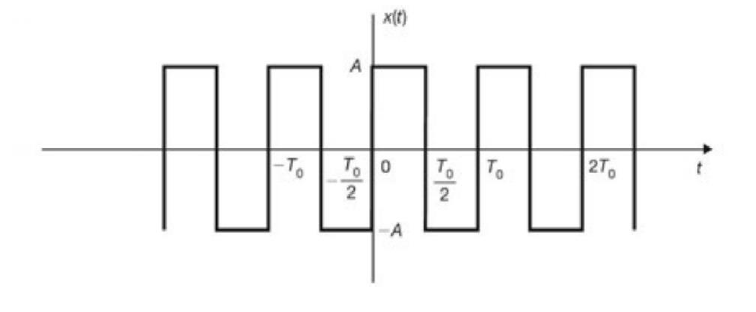
\includegraphics[width = 0.5 \textwidth]{images/3.png}
\end{center}


$$\omega_0 = \frac{2\pi}{T}$$

$$a_k = \frac{1}{T_0} \int_{-T_0/2}^{T_0/2} x(t) e^{-j k \frac{2\pi}{T_0} t} dt$$

برای $k=0$ به طور جداگانه محاسبه کرده و داریم:

$$\boxed{a_0 = \frac{1}{T_0} \int_{-T_0/2}^{T_0/2} x(t) dt = 0}$$

برای باقی موارد داریم:

$$a_k = \frac{1}{T_0} \int_{-T_0/2}^{T_0/2} x(t) e^{-j k \frac{2\pi}{T_0} t} dt = \frac{1}{T_0}(\int_{-T_0/2}^{0} (-A) e^{-j k \frac{2\pi}{T_0} t} dt + \int_{0}^{T_0/2} (A) e^{-j k \frac{2\pi}{T_0} t} dt )$$

$$= \frac{1}{T_0} (\frac{A T_0 j (-1 + e^{j k \pi})}{2 k \pi} + \frac{- A  T_0 j (1 - e^{j k \pi})}{2 k \pi})$$

$$\boxed{= \frac{A j e^{-j k \pi} (-1 + e^{j k \pi})^2}{2 k \pi}}$$


\subsubsection{بخش c}

دوره تناوب پایه $|\sin (x)|$ برابر $\pi$ است و عملا مانند $\sin$ مثبتی بین $0$ تا $\pi$ است که در همه تناوب‌هایش تکرار می‌شود. در نتیجه باید براساس این تناوب حل کرد.

$$a_k = \frac{1}{\pi} \int_{0}^{\pi} |\sin (x)| e^{- 2 j k x} dx = \frac{1}{\pi}\int_{0}^{\pi} \sin (x) e^{- 2 j k x} dx $$

برای ضریب $a_0$ داریم:

$$a_0 = \frac{1}{\pi} \int_{0}^{\pi} \sin (x) dx = \frac{2}{\pi}$$


برای سایر ضرایب داریم:

$$a_k = \frac{1}{\pi}\int_{0}^{\pi} \frac{1}{2 j} (e^{i x} - e^{-ix}) e^{- 2 j k x}  dx$$

$$=\frac{1}{2 \pi} \left(\frac{e^{-j (2 k-1) x}}{2 k-1}-\frac{e^{-j (2 k+1) x}}{2 k+1}\right)|_{0}^{\pi}$$

$$=\frac{1}{2\pi} \left(\frac{1}{2 k+1}-\frac{1}{2 k-1}\right)+\frac{1}{2\pi} \left(\frac{e^{-j \pi  (2 k-1)}}{2 k-1}-\frac{e^{-j \pi  (2 k+1)}}{2 k+1}\right)$$

$$=\boxed{\frac{1}{\pi}\frac{1+e^{-2 j \pi  k}}{1-4 k^2}}$$

\subsection{سوال سوم}

\subsubsection{بخش a}



$$x(t) = 
+-2j e^{-2j \omega_0 t}
+-1j e^{-1j \omega_0 t}
+1j e^{1j \omega_0 t}
+2j e^{2j \omega_0 t}
$$

$$=
-\frac{4}{2j}(e^{2j \omega_0 t} - e^{-2j \omega_0 t})
-\frac{2}{2j}(e^{j \omega_0 t} - e^{-j \omega_0 t})$$

$$\boxed{= -4 \sin(2 \omega_0 t) -2 \sin( \omega_0 t)}$$


\subsubsection{بخش b}

عبارت مورد نظر باید ما را به یاد سری فوریه قطار ضربه بیندازد.

$$\delta_{T_0} (t) = \sum_{k=-\infty}^{\infty} c_k e^{jk\omega_0 t}$$

برای ضرایب فوریه چنین چیزی داریم:
$$
c_{k}=\frac{1}{T_{0}} \int_{-T_{0} / 2}^{T_{0} / 2} \delta(t) e^{-j k \omega_{0} t} d t=\frac{1}{T_{0}}
$$

$$
\delta_{T_{0}}(t)=\sum_{k=-\infty}^{\infty} \delta\left(t-k T_{0}\right)=\frac{1}{T_{0}} \sum_{k=-\infty}^{\infty} e^{j k \omega_{0} t} \quad \omega_{0}=\frac{2 \pi}{T_{0}}
$$


با توجه به این موضوع برای چیزی که در صورت سوال داده شده، می‌توانیم آن را معادل با 

$$
z(t)=\sum_{k=-\infty}^{\infty} e^{j k \omega_{0} t} \delta(t-T_0 k+2 k)
$$

بدانیم.

در عبارت بالا $2k$ برای زوج سازی و سپس $e$ برای شیفت فرکانسی اضافه شده است که باعث بشود که تنها عبارت‌های فرد $1$ بمانند و عبارت‌های زوج $0$ شوند.



\newpage

\subsection{سوال چهارم}

در سوال نمادهای $e_k$ و $d_k$ استفاده شده است ولی برای راحتی کار و از آن جایی که کلا دو سیگنال اصلی داریم، از $a_k$ و $b_k$ در جواب استفاده شده است.

$$
x_1[n] x_2[n]=\sum_{k=0}^{N_0-1} \sum_{l=0}^{N_0-1} a_{k} b_{l} e^{j(2 \pi / N_0)(k+l) n}
$$

$$
x_1[n] x_2[n]=\sum_{k=0}^{(N_0-1)} \sum_{l^{\prime}=k}^{(k+N_0-1)} a_{k} b_{l^{\prime}-k} e^{j(2 \pi / N_0)^{\prime} n}
$$

با توجه به متناوب بودن
$b_{l' -k}$
و
$e^{j 2\pi /N_0 l' n}$
داریم:

$$
x_1[n] x_2[n]=\sum_{k=0}^{N_0-1} \sum_{l^{\prime}=0}^{N_0-1} a_{k} b_{l^{\prime}-k} e^{j(2 \pi / N_0) t^{\prime} n}=\sum_{l=0}^{N_0-1}\left[\sum_{k=0}^{N_0-1} a_{k} b_{l-k}\right] e^{j(2 \pi / N_0) l n}
$$

پس

$$
c_{k}=\sum_{t=0}^{N_0-1} a_{k} b_{l-k}
$$

و معادلا:
$$
c_{k}=\sum_{k=0}^{N_0-1} b_{k} a_{l-k}
$$

برای اثبات رابطه پارسوال داریم:


$$
N_0 \sum_{l=\langle N_0\rangle} a_{l} b_{k-l}=\sum_{\langle N_0\rangle} x_1[n] x_2[n] e^{-j(2 \pi / N_0) k n}
$$

با قرار دادن $k=0$ داریم:

$$
N_0 \sum_{l=\langle N_0\rangle} a_{l} b_{-1}=\sum_{n= \langle N_0\rangle} x_1[n] x_2[n]
$$

در نتیجه:

$$
\frac{1}{N_{0}} \sum_{n=0}^{N_{0}-1} x[n]=\sum_{k=0}^{N_{0}-1} a_{k} b_{-k}
$$

\newpage
\subsection{سوال پنجم}

در نتیجه سوال قبل قرار می‌دهیم:

$$x_2[n] = x^*_1[n]$$

در نتیجه این موضوع داریم:

$$b_k = a^*_{-k}$$

پس

$$
\frac{1}{N_{0}} \sum_{n=0}^{N_{0}-1} x[n]=\sum_{n=0}^{N_{0}-1} a_{k} b_{-k}
$$

$$
\frac{1}{N_{0}} \sum_{n=0}^{N_{0}-1} x_1[n] x_1^*[n]=\sum_{k=0}^{N_{0}-1} a_{k} a^*_{k}
$$

بنابراین:

$$
\sum_{k=\langle n_0\rangle}\left|a_{k}\right|^{2}=\frac{1}{N_0} \sum_{n=\langle N_0\rangle}|x[n]|^{2} .
$$

\newpage
\subsection{سوال ششم}
$$
f(t)=\left\{\begin{array}{lc}
	t+\frac{5}{3} & -1 \leq t<0 \\
	-t+\frac{5}{3} & 0 \leq t<2 \\
	0 & 2 \leq t<4
\end{array}\right.
$$

\subsubsection{بخش a}
$$a_0 = \frac{1}{5} \int f(t) dt = \frac{1}{5}( \int_{-1}^{0} t + 5/3 dt  + \int_{0}^{2} -t + 5/3 dt )$$
$$= \frac{1}{5}(\frac{7}{6} + \frac{4}{3}) =\boxed{ \frac{1}{2}}$$

$$a_k = \frac{1}{5} \int_{-1}^{5} f(t) e^{-j k \frac{2\pi}{5} t} dt = \frac{1}{5} (\int_{-1}^{0} (t+\frac{5}{3}) e^{-j k \frac{2\pi}{5} t} dt + \int_{0}^{2} (-t+\frac{5}{3}) e^{-j k \frac{2\pi}{5} t} dt)$$


$$\frac{1}{5} (\frac{50 i \pi  k+e^{\frac{2 i \pi  k}{5}} (-75-20 i \pi  k)+75}{12 \pi ^2 k^2} + \frac{-50 i \pi  k+e^{\frac{-4}{5} i \pi  k} (-75-10 i \pi  k)+75}{12 \pi ^2 k^2})$$$$ = \frac{e^{\frac{1}{5} (-4) i \pi  k} \left(-2 i \pi  k+30 e^{\frac{4 i \pi  k}{5}}+e^{\frac{6 i \pi  k}{5}} (-15-4 i \pi  k)-15\right)}{12 \pi ^2 k^2} $$


یا اگر روش فرمول کسینوس و سینوس را برویم داریم:


$$a_n = \frac{2}{5} \int (f(t) \cos (\frac{2\pi}{5} n t)) dt$$
$$ =\frac{2}{5} (\int_{-1}^{0} (t+5/3) \cos(\frac{2 \pi}{5} n t) dt + \int_{0}^{2} (-t + 5/3) \cos (\frac{2 \pi}{5} n t) dt)$$
$$= \frac{\sin ^2\left(\frac{\pi  n}{5}\right) \left(4 \pi  n \sin \left(\frac{2 \pi  n}{5}\right)+30 \cos \left(\frac{2 \pi  n}{5}\right)+45\right)}{3 \pi ^2 n^2}$$


$$b_n = \frac{2}{5} (\int (f(t) \sin (\frac{2\pi}{5} n t)) dt$$
$$ =\frac{2}{5}( \int_{-1}^{0} (t+5/3) \sin(\frac{2 \pi}{5} n t) dt + \int_{0}^{2} (-t + 5/3) \sin (\frac{2 \pi}{5} n t) dt)$$
$$= \frac{15 \left(\sin \left(\frac{2 \pi  n}{5}\right)-\sin \left(\frac{4 \pi  n}{5}\right)\right)+4 \pi  n \cos \left(\frac{2 \pi  n}{5}\right)+2 \pi  n \cos \left(\frac{4 \pi  n}{5}\right)}{6 \pi ^2 n^2}$$



$$f(x) = a_0 + \sum_{n=1}^{N} (a_n \cos (n x) + b_n \sin (n x))$$




\subsubsection{بخش b}

کدهای مسئله به زبان پایتون در فایل 
\lr{\Verb+P1\_Q6\_b.py+}
موجود است و جواب قسمت‌های بعد براساس آن تولید شده است:

جملات مد نظر در ادامه نوشته شده اند. توجه کنید که به دلیل ویژگی‌های اعداد Floating-Point عموما ضرایبی که صفر بوده‌اند به صورت عددی ضربدر $10^{-33}$ نوشته شده‌اند.

پس از آن ابتدا در یک شکل سیگنال‌ها به ازای مقادیر $N$ به صورت جداگانه رسم شده‌اند. سپس در اشکال بعدی، به ازای هر کدام از مقادیر، نمودار آن با رنگ نارنجی روی نمودار اصلی با رنگ آبی رسم شده است.



$$a_{ 1 } = 0.772711906482877 , b_{ 1 } = 0.07175375986881644$$

$$a_{ 2 } = 0.27113541693643917 , b_{ 2 } = 0.028002784979373037$$

$$a_{ 3 } = -0.004852111911900812 , b_{ 3 } = -0.08960735823011712$$

$$a_{ 4 } = 0.004714960180721709 , b_{ 4 } = -0.010817086948420714$$

$$a_{ 5 } = 1.5195743635847465e-33 , b_{ 5 } = 0.06366197723675814$$

$$a_{ 6 } = 0.04083290139095018 , b_{ 6 } = -0.0008212742065860439$$

$$a_{ 7 } = 0.04515821107548206 , b_{ 7 } = -0.011886611106858576$$

$$a_{ 8 } = -0.01831062003374954 , b_{ 8 } = -0.023451895441009625$$

$$a_{ 9 } = -0.007676952848145469 , b_{ 9 } = -0.00338756817877342$$

$$a_{ 10 } = 1.5195743635847456e-33 , b_{ 10 } = 0.03183098861837907$$

$$a_{ 11 } = 0.017911214823682062 , b_{ 11 } = -0.0010816983697769051$$

$$a_{ 12 } = 0.023201132067024215 , b_{ 12 } = -0.008867354363816892$$

$$a_{ 13 } = -0.013610002113093692 , b_{ 13 } = -0.012990392854308745$$

$$a_{ 14 } = -0.006730131246383232 , b_{ 14 } = -0.0019169012948294058$$

$$a_{ 15 } = 1.5195743635847434e-33 , b_{ 15 } = 0.021220659078919374$$

$$a_{ 16 } = 0.01118956850490962 , b_{ 16 } = -0.000907051304878608$$

$$a_{ 17 } = 0.015464268832541013 , b_{ 17 } = -0.006821294507069879$$

$$a_{ 18 } = -0.010581176024894123 , b_{ 18 } = -0.008919232952258454$$

$$a_{ 19 } = -0.005585535368095415 , b_{ 19 } = -0.0013214190722783403$$

$$a_{ 20 } = 1.5195743635847419e-33 , b_{ 20 } = 0.015915494309189534$$

$$a_{ 21 } = 0.008076648709406326 , b_{ 21 } = -0.0007562919849315991$$

$$a_{ 22 } = 0.011564843734622392 , b_{ 22 } = -0.005507870241109013$$

$$a_{ 23 } = -0.008613443680564381 , b_{ 23 } = -0.006775588961597922$$

$$a_{ 24 } = -0.004711199325475308 , b_{ 24 } = -0.0010040831881916652$$

$$a_{ 25 } = 1.5195743635847393e-33 , b_{ 25 } = 0.012732395447351627$$

$$a_{ 26 } = 0.006300406249170883 , b_{ 26 } = -0.0006432609418058376$$

$$a_{ 27 } = 0.009225781951316991 , b_{ 27 } = -0.004609416023114295$$

$$a_{ 28 } = -0.007250921405575788 , b_{ 28 } = -0.005457578628620997$$

$$a_{ 29 } = -0.004055794714702865 , b_{ 29 } = -0.0008081706869254678$$

$$a_{ 30 } = 1.519574363584735e-33 , b_{ 30 } = 0.010610329539459687$$

$$a_{ 31 } = 0.005157489248731366 , b_{ 31 } = -0.0005579230259798711$$

$$a_{ 32 } = 0.007669732145959915 , b_{ 32 } = -0.003959686879886606$$

$$a_{ 33 } = -0.006256136875045252 , b_{ 33 } = -0.004566755490351168$$

$$a_{ 34 } = -0.003553802680498653 , b_{ 34 } = -0.0006755979057181989$$

$$a_{ 35 } = 1.5195743635847316e-33 , b_{ 35 } = 0.009094568176679736$$

$$a_{ 36 } = 0.004362360888597353 , b_{ 36 } = -0.0004918855395621645$$

$$a_{ 37 } = 0.006561005399865466 , b_{ 37 } = -0.0034690828700930944$$

$$a_{ 38 } = -0.005499407016535415 , b_{ 38 } = -0.0039249666296024815$$

$$a_{ 39 } = -0.003159413834482431 , b_{ 39 } = -0.0005800860028377107$$

$$a_{ 40 } = 1.5195743635847268e-33 , b_{ 40 } = 0.007957747154594767$$

$$a_{ 41 } = 0.003778044173238204 , b_{ 41 } = -0.00043950225495442116$$

$$a_{ 42 } = 0.005731421240004929 , b_{ 42 } = -0.003085957785323703$$

$$a_{ 43 } = -0.004905005087522983 , b_{ 43 } = -0.0034408366129256586$$

$$a_{ 44 } = -0.0028423248893797424 , b_{ 44 } = -0.0005080735752180709$$

$$a_{ 45 } = 1.5195743635847215e-33 , b_{ 45 } = 0.00707355302630646$$

$$a_{ 46 } = 0.0033308907366752464 , b_{ 46 } = -0.00039703351695859266$$

$$a_{ 47 } = 0.0050875680137263376 , b_{ 47 } = -0.0027786711713284526$$

$$a_{ 48 } = -0.004426026511190478 , b_{ 48 } = -0.003062743915561243$$

$$a_{ 49 } = -0.0025822630276678576 , b_{ 49 } = -0.0004518742494494454$$

$$a_{ 50 } = 1.5195743635847159e-33 , b_{ 50 } = 0.006366197723675813$$


\begin{center}
	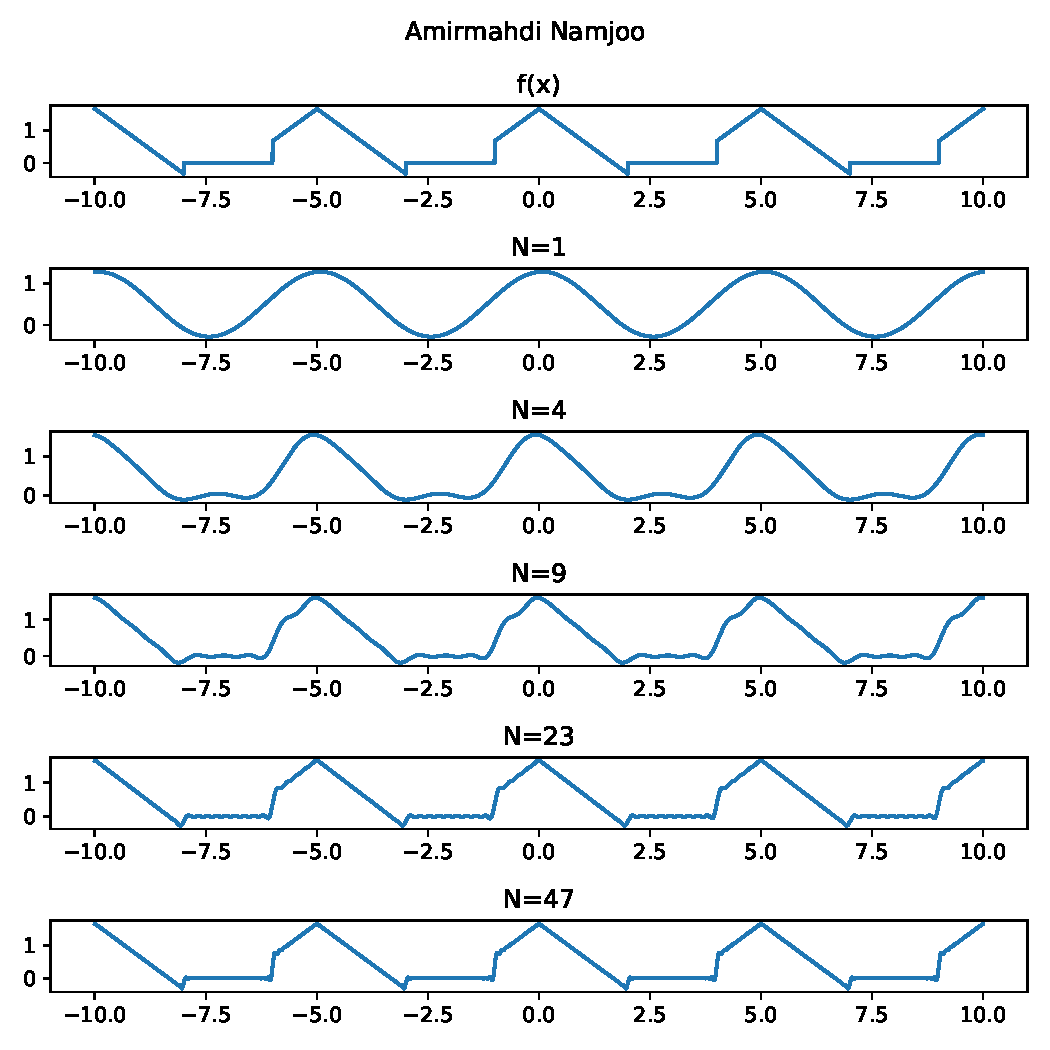
\includegraphics[width = 1.0 \textwidth]{images/6-1.pdf}
\end{center}



\begin{center}
	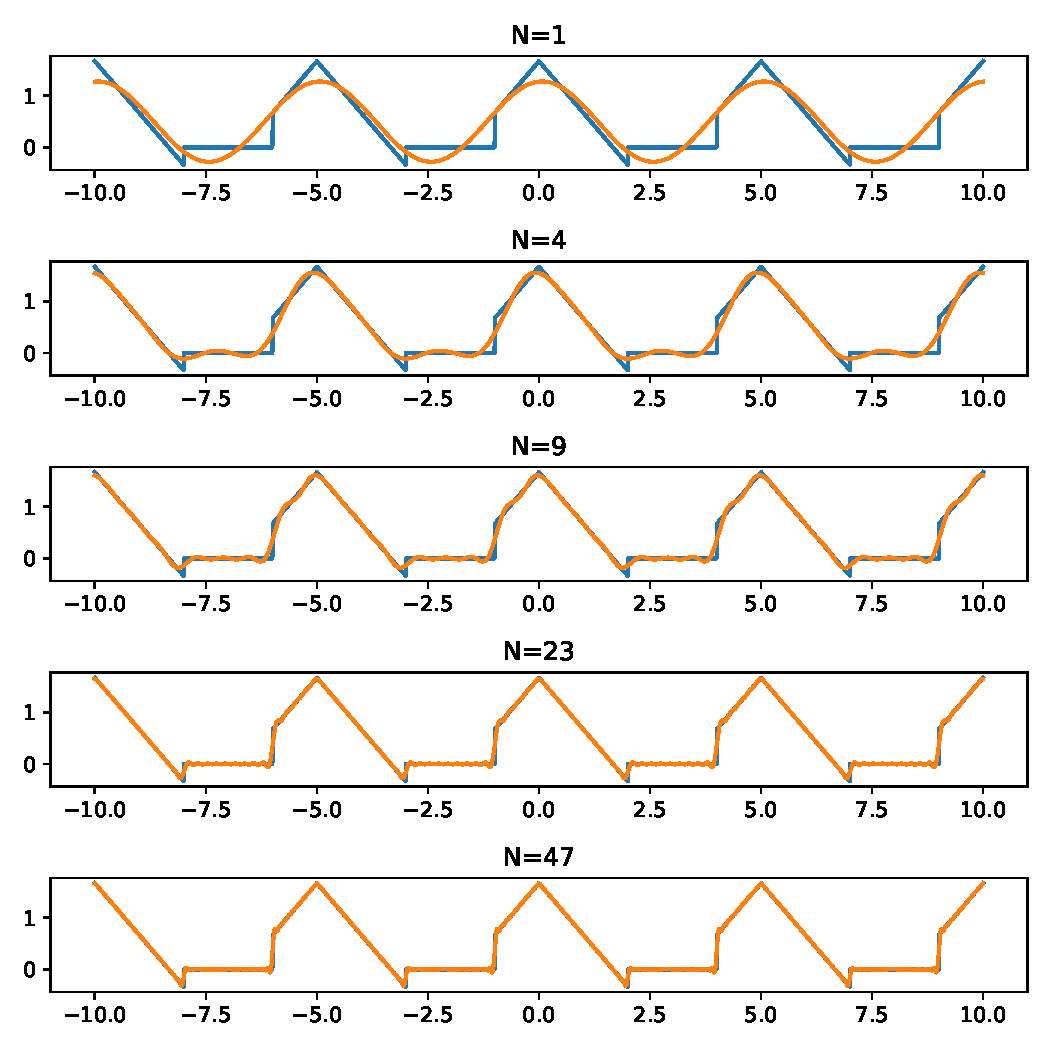
\includegraphics[width = 1.0 \textwidth]{images/6-2.pdf}
\end{center}

\subsubsection{بخش c}

کد این بخش در فایل
\lr{\Verb+P1\_Q6\_c+}
قرار دارد.



\begin{center}
	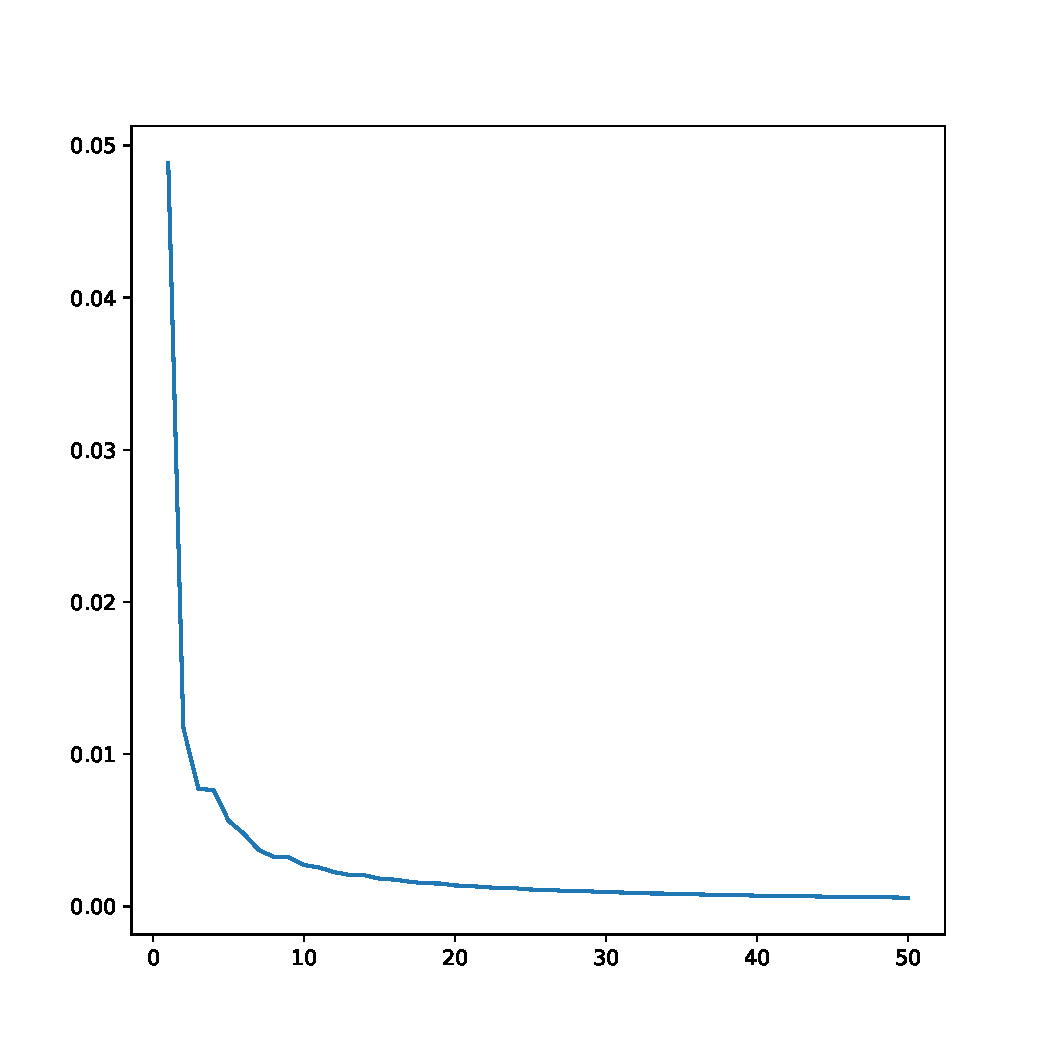
\includegraphics[width = 1.0 \textwidth]{images/6-3.pdf}
\end{center}

\newpage
\section{تبدیل فوریه}

\subsection{سوال اول}

$$X(jw) = \int_{-\infty}^{\infty} x(t) e^{-j \omega t} dt$$

\subsubsection{بخش a}

$$e^{- a |t|} \sin \omega_0 t$$

$$X(jw) = \int_{-\infty}^{\infty} e^{- a |t|} \sin (\omega_0 t) e^{-j \omega t}  dt$$
$$\int_0^{\infty}  \sin (\omega_0 t) e^{(-jw -a) t} + \int_{-\infty}^{0}  \sin (\omega_0 t) e^{(-jw + a)t}$$

$$= \int_{0}^{\infty} e^{-at} \sin(\omega_0 t) (e^{-jwt} - e^{jwt})$$

$$= -2j \int_{0}^{\infty} e^{at} \sin(\omega_0 t) \sin(\omega t)$$


$$= j \int_{0}^{\infty} e^{at} (\cos ((\omega_0 + \omega) t) - \cos((\omega_0 - \omega )t))$$

$$= j(e^{a t} \left(\frac{a \cos (t (\omega_0-\omega))+(\omega_0-\omega) \sin (t (\omega_0-\omega))}{a^2+(\omega_0-\omega)^2}-\frac{a \cos (t (\omega_0+\omega))+(\omega_0+\omega) \sin (t (\omega_0+\omega))}{a^2+(\omega_0+\omega)^2}\right))|_{0}^{\infty}$$

با شرط $a<0$ داریم:

$$= \frac{4 a \omega_0 \omega j}{\left(a^2+\omega_0^2\right)^2+2 \omega^2 (a-\omega_0) (a+\omega_0)+\omega^4}$$

\newpage


\subsubsection{بخش b}

$$
X(j \omega)=\int_{-1}^{1}(1+\cos (\pi t)) e^{-j \omega t} d t
$$

$$
\begin{gathered}
	X(j \omega)=\int_{-1}^{1} e^{-j \omega t} d t+\int_{-1}^{1} \frac{e^{j \pi t}+e^{-j \pi t}}{2} e^{-j \omega t} d t \\
	X(j \omega)=\left.\frac{e^{-j \omega t}}{-j \omega}\right|_{-1} ^{1}+\left.\frac{1}{2}\left(\frac{e^{j(\pi-\omega)}}{j(\pi-\omega)}+\frac{e^{-j(\pi+\omega) t}}{-j(\pi+\omega)}\right)\right|_{-1} ^{1} \\
	X(j \omega)=\frac{e^{-j \omega}-e^{j \omega}}{-j \omega}+\frac{1}{2}\left(\frac{e^{j(\pi-\omega)}-e^{j(\pi-\omega)}}{j(\pi-\omega)}+\frac{e^{-j(\pi+\omega)}-e^{j(\pi+\omega)}}{-j(\pi+\omega)}\right) \\
	X(j \omega)=\frac{2}{\omega} \cdot \frac{e^{j \omega}-e^{-j \omega}}{2 j}+\frac{1}{\pi-\omega} \cdot \frac{e^{j(\pi-\omega)}-e^{j(\pi-\omega)}}{2 j}+\frac{1}{\pi+\omega} \cdot \frac{e^{j(\pi+\omega)}-e^{-j(\pi+\omega)}}{2 j} \\
	X(j \omega)=\frac{2 \sin \omega}{\omega}+\frac{\sin (\pi-\omega)}{\pi-\omega}+\frac{\sin (\pi+\omega)}{\pi+\omega}
\end{gathered}
$$

$$\boxed{X(j\omega) = \frac{2 \sin \omega}{\omega}+\frac{\sin (\pi-\omega)}{\pi-\omega}+\frac{\sin (\pi+\omega)}{\pi+\omega}}$$

\subsubsection{بخش c}


می‌دانیم تبدیل فوریه $e^{a|t|}$ به صورت
$\frac{2a}{a^2 + \omega^2}$
است.
اثبات:

$$
\begin{gathered}
	x(t)=e^{-d t \mid}=\left\{\begin{array}{ll}
		e^{-a t} & t>0 \\
		e^{a t} & t<0
	\end{array}\right. \\
	X(\omega)=\int_{-\infty}^{0} e^{a t} e^{-j \omega t} d t+\int_{0}^{\infty} e^{-a t} e^{-j \omega t} d t \\
	=\int_{-\infty}^{0} e^{(a-j \omega) t} d t+\int_{0}^{\infty} e^{-(a+j \omega) t} d t \\
	=\frac{1}{a-j \omega}+\frac{1}{a+j \omega}=\frac{2 a}{a^{2}+\omega^{2}}
\end{gathered}
$$

همچنین می دانیم که تبدیل فوریه
$t f(t)$
تبدیل فوریه برابر است با:
$j \frac{d}{d\omega} F(\omega)$

پس در این جا هم جواب

$$j \frac{d}{d \omega } \frac{2a}{a^2 + \omega^2} = -\frac{4 a  j \omega}{\left(a^2+\omega^2\right)^2}$$


\subsubsection{بخش d}

$$X(jw) = \int_{-\infty}^{\infty} \cos (\omega_0 t) u(t) e^{-j \omega t} dt$$

$$X(jw) = \int_{0}^{\infty} \cos (\omega_0 t) e^{-j \omega t} dt$$

$$X(jw) = \frac{1}{2} \int_{0}^{\infty} (e^{j \omega_0 t} + e^{-j \omega_0 t}) e^{-j \omega t} dt$$
$$= -\frac{j \omega}{\omega^2-{\omega_0}^2}$$


\subsubsection{بخش e}

$$
\Delta(t)=\left\{\begin{array}{lr}
	1-2|t| & 0 \leq t \leq 1 / 2 \\
	0 & \text { otherwise }
\end{array}\right. = 
\left\{\begin{array}{lr}
	1-2t & 0 \leq t \leq 1 / 2 \\
	0 & \text { otherwise }
\end{array}\right.
$$


$$
\begin{aligned}
	F(\omega) &=\int_{-\infty}^{\infty} \Delta(t) e^{-j \omega t} d t \\
	&=\int_{0}^{1 / 2}(1-2 t) e^{-j \omega t} d t \\
	&=\left.\frac{j \omega(2 t-1)+2}{(j \omega)^{2}} e^{-j \omega t}\right|_{t=0} ^{1 / 2} \\
	&=\frac{2-j \omega-2 e^{-j \omega / 2}}{\omega^{2}}
\end{aligned}
$$

\subsubsection{بخش f}

$$
x(t)=\left\{\begin{aligned}
	1 & \text { if } 1 \leq|t| \leq 3 \\
	-1 & \text { if }|t|<1 \\
	0 & \text { otherwise }
\end{aligned}\right.
$$

می‌دانیم که تبدیل فوریه سیگنال مستطیلی بین $-1/2$ تا $1/2$ به صورت:
$\frac{\sin \frac{\omega }{2}}{\frac{\omega}{2}} = sinc (\omega/2)$
است. اگر سیگنال مستطیلی ذکر شده را با نماد $\Pi(t)$ نمایش بدهیم، عبارت بالا
$\Pi(t/6) - 2\Pi (t/2)$
است. در نتیجه
$$F(\omega) = 6sinc(6 \omega/2) - 4 sinc(2 \omega /2) = 6sinc(3\omega) - 4 sinc(\omega)$$

\newpage

\subsection{سوال دوم}

\subsubsection{بخش a}

$$
F(\omega)=\frac{16-16 j \omega+4 \omega^{2}-4 j \omega^{3}}{54+81 j \omega+18 \omega^{2}+31 j \omega^{3}-6 \omega^{4}}
$$

$$F(\omega) = \frac{4 (-2 + j\omega) (-1 + j\omega) (2 + j\omega)}{-(3 + j\omega)^2 (-3 + 2 j\omega) (2 + 3 j\omega)}$$

$$= \frac{80}{63 (j\omega+3)^2}+\frac{28}{1053 (2 j\omega-3)}+\frac{640}{637 (3 j\omega+2)}-\frac{4028}{3969 (j\omega+3)}$$

$$\frac{80}{63} t e^{-3t} u(t) +\frac{-14}{1053}e^{\frac{3}{2}t}u(-t)+\frac{640}{1911}e^{\frac{-2}{3} t}u(t) + \frac{4028}{3969} e^{-3t}u(t) $$

\subsubsection{بخش b}

$$F(j\omega) = 2\pi j \omega e^{-|\omega|}$$


$$x(t) =\frac{1}{2\pi}\int_{-\infty}^{\infty} 2\pi j \omega e^{-|\omega|} e^{j \omega t} d \omega$$

$$ \int_{-\infty}^{0} j\omega e^{\omega} e^{j \omega t} d\omega + \int_{0}^{\infty} j\omega e^{-\omega} e^{j\omega t} d\omega$$

$$=\frac{i}{(t-i)^2} +(-\frac{i}{(t+i)^2}) $$

$$=-\frac{4 t}{\left(t^2+1\right)^2}$$

\newpage
\subsection{سوال سوم}
\newpage

\subsection{سوال چهارم}

$$h(t)=\frac{\sin (10 \pi  t)-\sin (6 \pi  t)}{2 \pi  t}$$

$$H(j\omega) = 
\left\{\begin{array}{ll}
	\frac{1}{2}, & |\omega|<10\pi \\
	0, & |\omega|>10\pi
\end{array}\right.
 -
 \left\{\begin{array}{ll}
 	\frac{1}{2}, & |\omega|<6\pi \\
 	0, & |\omega|>6\pi
 \end{array}\right.
 $$
 
 
 $$x(t) = \frac{1}{2} (\cos (5 \pi  t)+\cos (9 \pi  t))$$
 
 
 $$X(j\omega) = \frac{\pi}{2} (\delta(\omega-5\pi) + \delta(\omega + 5\pi)) + \frac{\pi}{2} (\delta(\omega-9\pi) + \delta(\omega + 9\pi))$$
 
 با ضرب $H$ در $X$ ، عبارت داری $5\pi$ که فقط در $5\pi$ مقدار دارد، در هر دو حالت $H$ شامل حالت $\frac{1}{2}$ شده و صفر می‌شود. ولی عبارت دومی فقط در حالت $|w|<10\pi$ صدق می‌کند و نصف می‌شود. در نتیجه:
 
 $$Y(j\omega) =\frac{\pi}{4} (\delta(\omega-9\pi) + \delta(\omega + 9\pi))$$
 
 پس
 
 $$y(t) = \frac{1}{4} \cos (9 \pi t)$$
 
 
\subsection{سوال پنجم}

$$
2 \frac{d^{2} y(t)}{d t^{2}}+3 \frac{d y(t)}{d t}-2 y(t)=x(t-1)
$$

با فرض شرایط اولیه صفر:

$$2 (j\omega)^2 Y(j\omega) + 3 (j\omega) Y(j\omega) - 2 Y(j\omega) = e^{-j\omega} X(j \omega)$$

$$X(j \omega) = \frac{1}{5 + j\omega} - \frac{1}{1 +j \omega}$$


$$Y(j \omega) = e^{- j \omega} \times \frac{\frac{1}{j\omega+5}-\frac{1}{j\omega+1}}{2 j\omega^2+3 j\omega-2}$$

$$= e^{-j \omega}\times( -\frac{4}{(j\omega+1) (j\omega+5) \left(2 j\omega^2+3 j\omega-2\right)})$$
$$= e^{-j \omega} \times( -\frac{4}{15 (j\omega+2)}+\frac{1}{33 (j\omega+5)}-\frac{32}{165 (2 j\omega-1)}+\frac{1}{3 (j\omega+1)})$$

ابتدا قسمت درون پرانتز را تبدیل فوریه معکوس می گیریم:

$$\rightarrow \frac{-4}{15} e^{-2t}u(t) + \frac{1}{33} e^{-5t}u(t) + \frac{16}{65} e^{\frac{1}{2} t} u(-t) + \frac{1}{3} e^{-t}u(t) $$

حال اثر $e^{-j \omega}$ را که شییفت به راست می دهد را اعمال می‌کنیم:


$$y(t) = \frac{-4}{15} e^{-2(t-1)}u(t-1) + \frac{1}{33} e^{-5(t-1)}u(t-1) + \frac{16}{65} e^{\frac{1}{2} (t-1)} u(-(t-1)) + \frac{1}{3} e^{-(t-1)}u(t-1) $$
$$=\frac{-4}{15} e^{-2t+2)}u(t-1) + \frac{1}{33} e^{-5t+5)}u(t-1) + \frac{16}{65} e^{\frac{1}{2} t-\frac{1}{2}} u(-t+1) + \frac{1}{3} e^{-t+1}u(t-1)$$

\newpage
\subsection{سوال ششم}

$$
\sum_{k=-\infty}^{+\infty} \delta\left(\omega-k \omega_{0}\right)=\frac{1}{\omega_{0}} \sum_{n=-\infty}^{+\infty} e^{\frac{2 \pi n j \omega}{\omega_{0}}}
$$

اگر توجه کنیم عبارت صورت سوال به شدت شبیه سری فوریه است. در اصل عبارت
$\sum_{k=-\infty}^{+\infty} \delta\left(\omega-k \omega_{0}\right)$
یک عبارت متناوب با دوره تناوب $\omega_0$ است که در هر $\omega_0$ یک تابع ضربه ایجاد کرده است. در نتیجه ضرایب فوریه آن را در یک دوره تناوب بدست می‌آوریم. البته بهتر بود به جای نماد $\omega_0$ از نماد $T_0$ استفاده می‌شد چون عملا این جا $\omega_0$ فرکانس نیست و خود دوره تناوب است ولی به هر حال با همین نماد جلو می‌رویم. عملا بهتر بود برای رعایت نمادگذاری به جای $\omega$ هم $t$ گذاشته می‌شد ولی در صورت سوال نمادگذاری متفاوتی استفاده شده است و از آن جایی که عملا تبدیل خاصی هم خواسته نشده است، می‌توانیم به صورت سوال به چشم یک تابع معمولی نگاه کنیم که به جای نماد $t$ نماد $\omega$ در آن گذاشته شده است.

$$a_k = \frac{1}{\omega_0} \int_{-\omega_0/2}^{\omega_0/2} \sum_{n=-\infty}^{\infty} \delta (\omega - n \omega_{0} ) e^{-jk\frac{\omega_0}{2 \pi} \omega} d\omega$$

عبارت بالا فقط به ازای $n=0$ مقدار غیر صفر دارد (در بازه انتگرال نوشته شده):

$$a_k = \frac{1}{\omega_0} \int_{-\omega_0/2}^{\omega_0 /2} \delta(\omega) e^{-j k \frac{\omega_0}{2\pi}\omega}  d\omega$$

عبارت بالا تنها در $\omega=0$ ناصفر است پس:

$$a_k = \frac{1}{\omega_0} \int_{-\omega_{0}/2}^{\omega_0/2} \delta(\omega) d\omega = \frac{1}{\omega_0}$$

در نتیجه با توجه به رابطه سری فوریه به عبارت زیر می رسیم. توجه کنید که در این جا عملا
 $\omega_0$
  رابطه فوریه به صورت 
   $\frac{\omega_0}{2\pi}$
   و $t$ آن رابطه به صورت $\omega$ است.
   

$$\sum_{k=-\infty}^{+\infty} \delta\left(\omega-k \omega_{0}\right)= \sum_{n=-\infty}^{+\infty} a_n e^{\frac{2 \pi n j \omega}{\omega_{0}}}$$

$$\sum_{k=-\infty}^{+\infty} \delta\left(\omega-k \omega_{0}\right)=\frac{1}{\omega_{0}} \sum_{n=-\infty}^{+\infty} e^{\frac{2 \pi n j \omega}{\omega_{0}}}$$

\newpage
\subsection{سوال هفتم}

قضیه را به شکل کلی اثبات می‌کنیم.

تابع را با $f$ و تبدیل فوریه آن را با $F$ نشان می‌دهیم.

در این سوال اثبات می‌کنیم که $f$ و  $F$ نمی‌توانند همزمان support متناهی داشته باشند مگر این که $f=0$ باشد. یعنی به جز تابع $0$ که تبدیل فوریه‌ اش هم $0$ است و عملا می‌توان گفت support ای ندارد، هیچ حالتی دیگری امکان ندارد هردوی آن‌ها همزمان متناهی باشند. البته در اصل اثباتی که این جا می‌نویسیم، برای حالت compact-support است ولی  عملا compact-support حالت finite-support را هم پوشش می‌دهد. compact-support نشان دهنده وجود یک بازه است که در آن مقدار تابع ناصفر است و پس از آن صفر است و عملا تعداد support متناهی را حالت خاصی از compact-support بدانیم.



فرض کنیم که $f$ پیوسته بوده و در بازه
$[-\pi/2 , pi/2]$
تعریف شده باشد. همچنین 
$F(\omega)$
به ازای 
$|\omega|>N$
برابر صفر باشد. نشان می‌دهیم که چنین حالتی تنها در صورتی که $f$ صفر باشد امکان پذیر است. برای این کار، $f$ را به صورت متناوب در نظر گرفته و دوره تناوب آن را بین
$[-\pi , \pi]$
قرار می‌دهیم. در این صورت ضرایب سری فوریه آن به صورت زیر می‌شود:

$$c_n = \frac{1}{2\pi} (\int_{-\pi}^{\pi} f(x) e^{j n x} dx)$$
عبارت داخل پرانتز عملا خود تبدیل فوریه $f$ است. یعنی
$c_n = \frac{1}{2\pi} F(n)]$
شده است. حال اگر به ازای
$|n|>N$
مقادیر تبدیل فوریه صفر باشند، یعنی عبارت بالا هم تنها به ازای تعداد محدوی عدد مقدار ناصفر دارد.

در نتیجه یعنی سری فوریه $f$ در بازه 
$[-\pi , \pi]$
یک جمع متناهی به صورت
$$f(x)= \sum_{n=-N}^{n=N} c_n e^{j n x}$$
است. این عبارت عملا یک چندجمله ای مثلثاتی از درجه $N$ (یا کمتر از $N$) است.

البته توجه کنید که ممکن است ابهاماتی پیرامون همگرایی پیش بیاید ولی از آن جایی که 
$\sum_{n=-\infty}^{\infty} |c_n| <\infty$
است (به دلیل متناهی بودن) می توانیم از همگرایی مطمئن باشیم.

حال نشان می‌دهیم که یک تابع چند جمله ای مثلثاتی که بعد از یک بازه‌ای کاملا صفر می‌شود باید متحد با صفر باشد.


$$
P_{N}(x)=\sum_{-N}^{N} c_{n} e^{i n x}=
$$


$$
\left(\sum_{-N}^{N} \alpha_{n} \cos n x+\beta_{n} \sin n x\right)+i\left(\sum_{-N}^{N} A_{n} \cos n x+B_{n} \sin n x\right)
$$
$$=u(x) + i v(x)$$

از طرفی می‌دانیم که توابع مثلثاتی بسط تیلور همگرا دارند. در نتیجه اگر مقدار آن حول نقطه ای خاص $0$ باشد، همه ضرایب تیلور آن باید صفر باشند. در نتیجه با توجه به این که در مثلا بازه
 $[\pi/2 , \pi]$
 مقدار تابع صفر است و با توجه به همگرایی بسط تیلور تابع، مقدار آن باید به ازای همه نقاط صفر بوده باشد. یعنی $f\equiv0$ بوده است.
 
 در نتیجه از متناهی بودن support هر دوی $f$ و $F$ نتیجه گرفتیم که $f$ صفر است. در نتیجه امکان ندارد هر دوی آن‌ها متناهی باشند.
 
 توجه کنید که بازه انتخاب شده برای این سوال اختیاری بود و می‌شد بازه‌های دیگری را هم انتخاب کرد و به راحتی با Scale کردن مقادیر، همچنان توضیحات بالا برقرار بود.
 
 
 البته تقریبا بدیهی بود که یک چندجمله ای مثلثاتی درجه $N$ حداکثر $2N$ ریشه دارد (این را هم می‌شود به راحتی با در نظر گرفتن صفحه مختلط و نوشتن توابع مثلثاتی به صورت مختلط اثبات کرد) و در نتیجه این که در بازه
 $[\pi/2 , \pi]$
 عبارت تماما صفر بود و بسط مثلثاتی متناهی از آن داشتیم،‌ نشان دهنده این بود که این عبارت باید متحد با صفر باشد. توجیه بسط تیلور صرفا برای کامل تر شدن اثبات بود.
 
 
 توجه کنید که در صورت سوال \lr{finite} بودن صحبت شده که می توان آن را مشابه \lr{compact} بودن در نظر گرفت ولی با بازه گسترده تر. چون \lr{compact} بودن و \lr{support} هم بر این اساس است که از یک بازه ای به بعد، همه مقادیر صفر بشوند و قبل از لزوما صفر نباشند. در حالت \lr{compact} می‌تواند تعداد این مقادیر بیشمار هم باشد و مثلا یک بازه پیوسته باشد ولی می‌تواند محدود هم باشد و مشکل خاصی از این بابت نیست.
 
 \newpage
\section{سوال عملی}

\subsection{بخش ۱}

نشان می‌دهیم که تبدیل معکوس فوریه گسسته به صورت زیر است:

$$x[n] = \frac{1}{N} \sum_{k=0}^{N-1} X_k e^{2\pi j k n / N}$$

که در آن $X_k$ خود تبدیل فوریه گسسته است.

برای اثبات داریم:

$$\frac{1}{N} \sum_{k=0}^{N-1} X_k e^{2\pi j k n /N} = \frac{1}{N} \sum_{k=0}^{N-1}(\sum_{m=0}^{N-1} x_m e^{- 2\pi j k m/N})e^{2 \pi j k n /N}$$

$$= \frac{1}{N}\sum_{m=0}^{N-1}\sum_{k=0}^{N-1} x_m e^{2\pi j k(n-m)/N} = \sum_{m=0}^{N-1} x_m (\frac{1}{N} \sum_{k=0}^{N-1} e^{2 \pi j (n-m)/N})$$
$$=\sum_{m=0}^{N-1} x_m \delta[n-m] = x_n$$

 
\end{document}



